\documentclass[tikz,border=5pt]{standalone}
\usetikzlibrary{patterns, calc, arrows.meta}

\begin{document}

% Figure 12a: Stable Model Polytope (Surgery Triangles)
% Matches precise topology of sketch_12
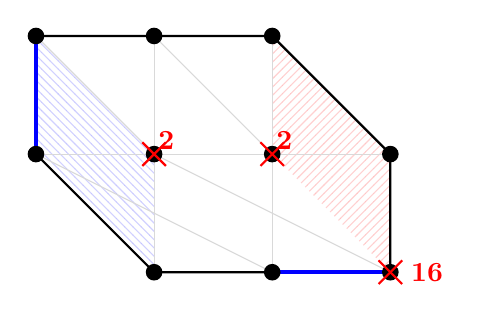
\begin{tikzpicture}[scale=1.5]
    % Define the 10-node lattice grid
    \coordinate (T1) at (0, 2); \coordinate (T2) at (1, 2); \coordinate (T3) at (2, 2);
    \coordinate (M1) at (0, 1); \coordinate (M2) at (1, 1); \coordinate (M3) at (2, 1); \coordinate (M4) at (3, 1);
    \coordinate (B1) at (1, 0); \coordinate (B2) at (2, 0); \coordinate (B3) at (3, 0);

    % 1. Surgery Triangles (Shaded regions)
    % Resting on boundary edges as per integral-affine surgery rules
    \fill[pattern=north west lines, pattern color=blue!30, opacity=0.6] (T1) -- (M1) -- (M2) -- cycle; % Top-left
    \fill[pattern=north west lines, pattern color=blue!30, opacity=0.6] (B1) -- (M1) -- (M2) -- cycle; % Bottom-left
    \fill[pattern=north east lines, pattern color=red!30, opacity=0.6] (T3) -- (M3) -- (M4) -- cycle; % Top-right
    \fill[pattern=north east lines, pattern color=red!30, opacity=0.6] (B3) -- (M3) -- (M4) -- cycle; % Bottom-right

    % 2. Full Lattice Grid/Triangulation (Light Gray)
    \begin{scope}[gray!30, thin]
        % Horizontal lines
        \draw (T1) -- (T3);
        \draw (M1) -- (M4);
        \draw (B1) -- (B3);
        % Vertical lines
        \draw (T2) -- (M2) -- (B1); % Shifted vertical
        \draw (T3) -- (M3) -- (B2); % Shifted vertical
        \draw (T1) -- (M1); 
        \draw (M4) -- (B3);
        % Triangulation Diagonals (down-right consistent with surgery)
        \draw (T1) -- (M2);
        \draw (T2) -- (M3);
        \draw (M1) -- (B2);
        \draw (M2) -- (B3);
    \end{scope}

    % 3. Polytope Boundary (Thick Solid Black)
    \draw[thick] (T1) -- (T3) -- (M4) -- (B3) -- (B1) -- (M1) -- cycle;

    % 4. Highlights (Blue Edges)
    \draw[ultra thick, blue] (T1) -- (M1); % Left boundary
    \draw[ultra thick, blue] (B2) -- (B3); % Bottom boundary

    % 5. Lattice Nodes (Black dots)
    \foreach \p in {T1,T2,T3,M1,M2,M3,M4,B1,B2,B3} {
        \fill (\p) circle (2pt);
    }

    % 6. Singular Nodes (Red Crosshairs + Labels)
    % Node "2" at M2 (1,1)
    \begin{scope}[shift={(M2)}]
        \draw[red, thick] (-0.1,-0.1) -- (0.1,0.1);
        \draw[red, thick] (-0.1,0.1) -- (0.1,-0.1);
        \node[red, font=\bfseries, above right=-2pt] {2};
    \end{scope}

    % Node "2" at M3 (2,1)
    \begin{scope}[shift={(M3)}]
        \draw[red, thick] (-0.1,-0.1) -- (0.1,0.1);
        \draw[red, thick] (-0.1,0.1) -- (0.1,-0.1);
        \node[red, font=\bfseries, above right=-2pt] {2};
    \end{scope}

    % Node "16" at B3 (3,0)
    \begin{scope}[shift={(B3)}]
        \draw[red, thick] (-0.1,-0.1) -- (0.1,0.1);
        \draw[red, thick] (-0.1,0.1) -- (0.1,-0.1);
        \node[red, font=\bfseries, right=4pt] {16};
    \end{scope}

\end{tikzpicture}

\end{document}
